\documentclass[a4paper, oneside, 11pt]{book}
\usepackage[utf8]{inputenc}
\usepackage[printonlyused]{acronym}

\newif\ifdraft
\drafttrue % Sagt aus, dass dieses Dokument ein Entwurf ist. Somit wird todonotes aktiviert. Zum deaktivieren diese Zeile auskommentieren oder auf \draftfalse setzen.

\newcommand{\documenttitle}{Installation und Konfiguration von Kata Containern zur Absicherung von medizinischen, personenbezogenen Daten in einer Contaienrplattform}
\newcommand{\documentsubtitle}{Praxisprojekt Bericht}
\newcommand{\documentsubject}{Bachelor of Sience, Software Engeneering}
\newcommand{\documentauthor}{Robin Bendix Müller, 70460210}
\newcommand{\documenttutor}{Herr Prof. Dr. Bernd Müller}
% In diesem Dokument werden die globalen \usepackage{}-Befehle eingefügt.
% Definition des Seitestils (Ränder, Schriftart, Abstände, usw.)

\usepackage[top=2.5cm, bottom=2cm, left=3cm, right=2cm]{geometry}

\usepackage[ngerman]{babel}
\selectlanguage{ngerman}

\usepackage[T1]{fontenc}

\usepackage[nottoc,notlot,notlof]{tocbibind}

\usepackage[bottom]{footmisc} % Fußnoten nach unten stellen

\setlength{\parindent}{0em} % Absatzeinrückung linksbündig
\usepackage{setspace}
\onehalfspacing
\usepackage{parskip}

\usepackage{graphicx}

\usepackage{etoolbox}
\makeatletter
\patchcmd{\@makechapterhead}{\vspace*{50\p@}}{}{}{} % Removes space above \chapter head
\patchcmd{\@makeschapterhead}{\vspace*{50\p@}}{}{}{} % Removes space above \chapter* head
\makeatother

\usepackage{fancyhdr}
\setlength{\headheight}{14.5pt}
\pagestyle{fancy}

\renewcommand{\chaptermark}[1]{
	\markboth{
		{\chaptername\ \thechapter\ #1}
	}{}
}

\renewcommand{\sectionmark}[1]{
	\markright{
		{\thesection\ #1}
	}
}

\fancypagestyle{titlepage}
{
	\setcounter{page}{-100000}
	\fancyhf{}
	\fancyfootoffset{0pt}
	\fancyheadoffset{0pt}
	\renewcommand{\headrulewidth}{0pt}
}


\usepackage{titlesec} % Im folgenden werden die Schriftarten der Überschriften gesetzt.
\titleformat{\chapter}[display] {\sffamily \huge}{\chaptertitlename\ \thechapter}{-5pt}{\Huge}
\titlespacing*{\chapter}{0pt}{0pt}{10pt}
\titleformat{\section}[display] {\sffamily \tiny}{}{0pt}{\LARGE \thesection\ }
\titlespacing*{\section}{0pt}{0pt}{0pt}
\titleformat{\subsection}[display] {\sffamily \tiny}{}{-15pt}{\Large \thesubsection\ }
\titlespacing*{\subsection}{0pt}{0pt}{0pt}
\titleformat{\subsubsection}[display] {\sffamily \tiny}{}{-15pt}{\large \thesubsubsection\ }
\titlespacing*{\subsubsection}{0pt}{0pt}{0pt}

\usepackage[titles]{tocloft}
\renewcommand{\cftchapfont}{\bf\sffamily}
\renewcommand{\cftsecfont}{\sffamily}
\renewcommand{\cftsubsecfont}{\sffamily}

\renewcommand{\cfttabfont}{\sffamily}
\renewcommand{\cftfigfont}{\sffamily}

\setcounter{secnumdepth}{3}

\usepackage{csquotes}
\usepackage[square, numbers]{natbib}

\usepackage[pdftex, pdfborder={0 0 0}]{hyperref}
\hypersetup{pdfauthor={\documentauthor},
	pdftitle={\documenttitle\ - \documentsubtitle},
	pdfsubject={\documentsubject},
	pdfkeywords={Betreuer:\ \documenttutor}}

\usepackage{lmodern}
\usepackage{listings}
\lstset{
	showspaces=false,
	showtabs=false,
	breaklines=true,
	showstringspaces=false,
	basicstyle=\ttfamily,
	frame=lt,
	rulecolor=\color{gray},
	framerule=3pt,
	xleftmargin=6pt,
}
\usepackage{color}
\usepackage{xcolor}
\usepackage{listings}
\usepackage{caption}

\newlength\myx
\setlength\myx{\textwidth}
\addtolength\myx{-2\fboxsep}

\DeclareCaptionFont{white}{\color{white} \sffamily}
\DeclareCaptionFormat{listing}{\colorbox{gray}{\parbox{\myx}{#1#2#3}}}
\captionsetup[lstlisting]{format=listing,labelfont=white,textfont=white}
\renewcommand{\lstlistingname}{Quelltext}

\setlength{\marginparwidth}{2cm}
\ifdraft
	\usepackage{todonotes}
\else
	\usepackage[disable]{todonotes}
\fi

%\usepackage{showframe} % Auskommentieren, um die Layoutgrenzen anzuzeigen


% In diesem Dokument wird die Silbentrennung eingefügt.

\begin{document}
	\listoftodos
	% Deckblatt
\frontmatter
\begin{titlepage}
	\thispagestyle{titlepage}
	\newgeometry{top=2cm, bottom=3.5cm, left=1.5cm, right=1.5cm}
	
	\hfill
	
\includegraphics[scale=0.93]{Bilder/ostfalia_logo.jpg}
	
	
\includegraphics[scale=1.20]{Bilder/reiter_wf_174mm.jpg}
	
	\hspace{1cm}
	\begin{minipage}{\dimexpr\textwidth-1.5cm\relax}
		{\Large\textsf{Fakultät Informatik}}
	\end{minipage}
	
	\vfil
	
	%-------------------------------------------------------------------------------
	\hspace{1cm}
	\begin{minipage}{\dimexpr\textwidth-1.5cm\relax}
		\hrulefill
		
		\vspace{2em}
		
		{\Large\textbf{\textsf{\documentsubject}}}
			
		\vspace{2em}
			
		{\Huge\textbf{\textsf{\documenttitle}}}
			
		\vspace{2em}
			
		{\Large\textsf{\documentsubtitle}}
		
		\vspace{1em}
		
		\hrulefill
	\end{minipage}	
	
	
	%-------------------------------------------------------------------------------
	\vfil
	
	\hspace{1cm}
	\begin{minipage}{\dimexpr\textwidth-1.5cm\relax}
		{\Large\textsf{Autor: \documentauthor}}
		
		\vspace{0.5cm}		
		
		{\Large\textsf{Betreuer: \documenttutor}}
	\end{minipage}
	
	\vspace{2em}
	
	%-------------------------------------------------------------------------------
	
	\enlargethispage{10\baselineskip}
	
	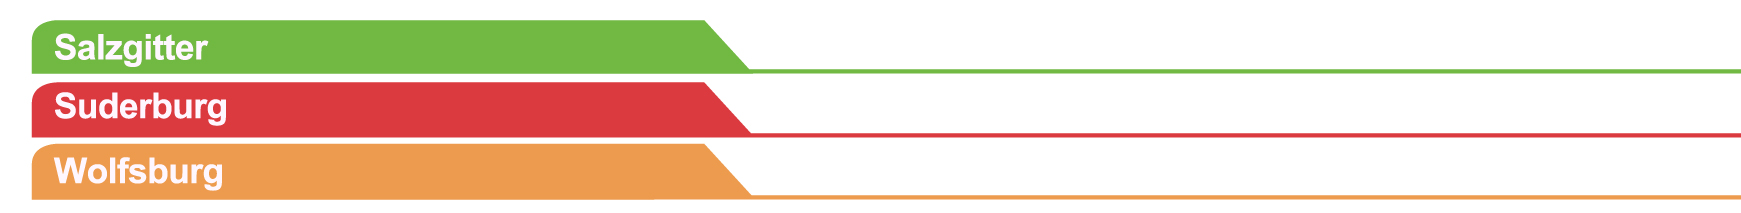
\includegraphics[scale=1.20]{Bilder/reiter_szsudwob_174mm.jpg}
	
	%*******************************************************************************
\end{titlepage}

\restoregeometry

	
	\tableofcontents
	\listoffigures
	\listoftables
	\pagebreak
	\thispagestyle{empty}
\chapter*{Abkürzungsverzeichnis}
\begin{acronym}[Bash]
    \acro{HZI}{Helmholtz Zentrum für Infektionsforschung}
    \acro{COVID-19}{Coronavirus SARS-CoV-2}
    \acro{SORMAS}{Surveillance, Outbreak Response Management and Analysis System}
    \acro{GA}{Gesundheitsamt}
    \acro{GAs}{Gesundheitsämter}
    \acro{SORMAS-ÖGD}{Sormas-ÖGD-Covid-19}
    \acro{VM}{Virtuelle Maschine}
    \acro{COP}{Container Orchestration Platform}
    \acro{OS}{Operating System}
    \acro{I/O}{input/output}
    \acro{OCI}{Open Container Initiative}
    \acro{runtime-spec}{Runtime Sepcification}
    \acro{image-spec}{Image Specification}
    \acro{CRI}{Container Runtime Interface}
    \acro{YAML}{YAML Ain't Markup Language}
    \acro{SSH}{Secure Shell}
    \acro{CNCF}{Cloud Native Computing Foundation}
    \acro{FOSS}{Free Open Source Software}
    \acro{OSF}{OpenStack Foundation}
    \acro{gRPC}{gRPC Remote Procedure Calls}
    \acro{DNS}{Dynamic Name Resolution}
    \acro{API}{Artificial Programming Interface}
    \acro{HTTP}{Hypertext Transfer Protocol}
    \acro{HTTPS}{Hypertext Transfer Protocol Secure}
    \acro{URL}{Uniform Resource Locator}
    \acro{SSL}{Secure Sockets Layer}
    \acro{TLS}{Transport Layer Security}
    \acro{PVC}{Persistent Volume Claim}
    \acro{PV}{Persistent Volume}
    \acro{NUC}{Next Level of Computing}
    \acro{PSU}{Power Supply Unit}
    \acro{PDU}{Power Distribution Unit}
    \acro{IP}{Internet Protocol}
    \acro{DHCP}{Dynamic Host Configuration Protocol}
    \acro{MAC}{Media Access Control}
    \acro{NAT}{Network Address Translation}
    \acro{KVM}{Kernel Virtual Machine}
    \acro{TOML}{Tom's Obvious, Minimal Language}
    \acro{regex}{regular expressions}
    \acro{TTL}{Time To Live}
    \acro{CNI}{Container Network Interface}
    \acro{CPU}{Central Processing Unit}
    \acro{S3}{Simple Storage Service}
    \acro{CRD}{Custom Resource Definition}
    \acro{DMZ}{demilitarized zone}
    \acro{GUI}{Graphical User Interface}
    \acro{DSGVO}{Datenschutz Grundverordnung}
\end{acronym}    



	\chapter*{Erklärung}

Hiermit versichere ich, dass ich die vorliegende Arbeit selbständig verfasst und keine anderen als die angegebenen Quellen und Hilfsmittel benutzt habe. Ich versichere, dass ich alle wörtlich oder sinngemäß aus anderen Werken übernommenen Aussagen als solche gekennzeichnet habe, und dass die eingereichte Arbeit weder vollständig noch in wesentlichen Teilen Gegenstand eines anderen Prüfungsverfahrens gewesen ist.

\vspace*{3em}

\newcommand*{\SignatureAndDate}[1]{
	\par\noindent\makebox[52mm]{\hrulefill}     \hfill\makebox[65mm]{\hrulefill}
	\par\noindent\makebox[52mm][l]{Ort, Datum}	\hfill\makebox[62mm][l]{#1}
}

\SignatureAndDate{Unterschrift}
	
	\mainmatter
	\chapter{Einleitung}

Die \ac{COVID-19} Pandemiesituation in Jahr 2020 stellte auf der ganzen Welt Gesundheitssysteme auf die Probe. 
Um das Virus bestmöglich bekämpfen zu können wurde das \ac{SORMAS}\footnote{2014 haben sich unter der Organisation des \ac{HZI} öffentliche Gesundheitsinstitutionen Deutschlands und Nigerias, sowie Forschungsinstitute und eine Software Entwicklungs Firma zusammengeschlossen um das Produkt \ac{SORMAS} zu entwickeln.
Die Software hatte den Zweck, den Ebola Ausbruch in Westafrika 2014/2015 einzudämmen.
In ihr können Fälle erfasst und gemanagt werden, um so Infektionsketten zu durchbrechen.
2016 wurde die Applikation zu einer Open Source Software migriert um die Unabhängigkeit von IT Firmen zu garantieren.
\cite{SORMAS_history}} vom \ac{HZI}\footnote{Das \ac{HZI} ist eine vom Bund finanzierte Instanz, an der Wissenschaftler alle möglichen Aspekte von Infektionskrankheiten untersuchen:
Wie werden diese ausgelöst und übertragen?
Wie werden sie vom Körper bekämpft?
Welche Wirkstoffe können bei der Infektionsbekämpfung hilfreich sein?
Warum sind einige Menschen anfälliger für Infektionskrankheiten als andere?
Mithilfe der Beantwortung dieser Fragen sollen Infektionskrankheiten im der aktuellen Zeit besser verstanden und bekämpft oder präventioniert werden. 
\cite{HZI_about}
\\
Aufgrund der Ausrichtung des \ac{HZI} beschäftiget sich das Institut im Jahr 2020 mit dem \ac{COVID-19}.} angepasst, um mit der Applikation nicht nur infizierte Personen managen zu können, sondern auch Kontaktpersonen zu erfassen.
Die neu entstandene Applikation bekam den Namen \ac{SORMAS-ÖGD} und wird vom Bund allen deutschen Gesundheitsämtern kostenlos zur Verfügung gestellt. 
\cite{SORMAS_covid}
\\
Deutschland hat insgesamt rund 400 \ac{GAs} \cite{GAs} von denen zum Zeitpunkt der Verfassung dieses Dokuments\footnote{07.10.2020} bereits 53 mit \ac{SORMAS-ÖGD} ausgestattet sind.
Diese Zahl nimmt jedoch stetig zu.  
An dieser Stelle kommt die Firma Netzlink~\ref{app:netzlink} ins Spiel: 
Die Firma hat durch eine Ausschreibung einen Vertrag mit dem Bund abgeschlossen, nach dem Netzlink jedem \ac{GA}, das interessiert ist, eine \ac{SORMAS-ÖGD}-Instanz zur Verfügung stellt.

\section{IST-Zustand}
Aktuell stellt Netzlink die \ac{SORMAS}-Instanzen auf ihrer VMWare\footnote{https://www.vmware.com/}-Infrastruktur zur Verfügung. 
\\
Die Daten, die in der \ac{SORMAS}-Datenbank gespeichert werden sind sogenannte besonders schützenswerte Daten.
\begin{quote}
    Bei Gesundheitsdaten gelten jedoch weitaus strengere Regeln als bei einfachen personenbezogenen Daten. 
    Gesundheitsdaten sind sensible, besonders schützenswerte Daten und werden im Gesetz als „besondere Kategorie“ personenbezogener Daten behandelt. 
    Grundsätzlich ist es untersagt, Gesundheitsdaten zu verarbeiten. 
    Dieses Verbot gilt nur dann nicht, wenn einer der gesetzlich geregelten Ausnahmefälle gegeben ist (Artikel 9 Abs. 2–4 \ac{DSGVO}). 
    \cite{Gesundheitsdatenschutz}
\end{quote}
Für die Netzlink als Provider der Applikation bedeutet das, dass die Daten der einzelnen \ac{GAs} streng getrennt werden müssen. 
Es dürfen nicht zwei Instanzen von \ac{SORMAS-ÖGD} auf der selben Maschine gehostet werden, da durch das Ausnutzen von Sicherheitslücken eventuell ein \ac{GA} die Daten eines Anderen einsehen könnte.
Um diese Abgrenzung zu garantieren rollt Netzlink mithilfe von Ansible\footnote{https://www.ansible.com/} für jedes \ac{GA} eine eigene \ac{VM} aus, um die Datensicherheit zu gewährleisten.
Auf der jeweiligen \ac{VM} werden dann mittels Docker \footnote{https://www.docker.com/} mehrere Container gestartet, die gemeinsam die \ac{SORMAS-ÖGD} Applikation darstellen.
\\
Für jedes \ac{GA} eine eigene VM zu bauen verbraucht unnötig viele Ressourcen:
\begin{itemize}
    \item Arbeitsspeicher für den Overhead der \ac{VM}
    \item Arbeitsspeicher und CPU Ressourcen um das Betriebssystem auf der \ac{VM} zu betreiben
    \item Zeit um die \ac{VM} auszurollen und zu starten 
\end{itemize}

\section{SOLL-Zustand}
Die ressourcenschonendere Lösung wäre, eine Containerplattform wie Kubernetes\footnote{https://kubernetes.io/} zu nutzen.
So kann viel Overhead eingespart werden, die Applikation kann schneller und zuverlässiger bereitgestellt werden. 
Die Abgrenzung, und damit der Schutz der Daten muss dabei unbedingt bestehen bleiben.

\section{Problemstellung}
Um den Schutz der besonders schützenswerten Daten zu garantieren muss eine Isolation geschaffen werden, die normalerweise bei einer Containerplattform nicht gegeben ist. 
Die Datenbank der verschiedenen \ac{GAs} dürfen nicht auf einer Maschine, also auf einem Kernel, laufen.
Diese Bedingungen können mit der Container Runtime "Kata-Containers"\footnote{https://katacontainers.io/} erfüllt werden. 
Die Funktionsweise dieser Runtime wird im Verlauf der Arbeit ausführlich erklärt. 
An dieser Stelle sei nur schon einmal vorweggenommen, dass diese Runtime die Prinzipien von \ac{VM}s und Containern  verbindet. 
Die "Container" die in dieser Runtime gestartet werden bekommen einen eigenen Kernel und sind daher eigentlich kleine \ac{VM}s, die sich jedoch wie Container anfühlen und bedienen lassen.
Hierbei wurde darauf geachtet, dass der Overhead der Instanzen so klein wie möglich gehalten wird, um das Container-Verhalten zu ermöglichen.
Die Aufgabenstellung ist also, eine Containerplattform aufzubauen die kata als Runtime nutzen kann.
Anschließend soll das bestehende \ac{SORMAS} mit seiner vollen Funktionalität auf Kubernetes migriert werden.

\section{Aufbau der Arbeit}
In Kapitel 2 werden die technischen Grundlagen, auf denen dieses Projekt aufbaut, erklärt. 
Hierbei wird kurz die Funktionsweise von Kubernetes angerissen, um die Integration von Kata-Containers in Kubernetes nachvollziehen zu können.
Die Unterschiede zwischen \ac{VM}s und und Containern werden herausgearbeitet und die Prinzipien der Kata-Runtime erklärt.
\\
Im Kapitel 3 wird der Aufbau und die Konfiguration des Clusters behandelt, dieses gliedert sich in:
\begin{itemize}
    \item Hardware Konfiguration
    \item Vorbereitung des Maschinen
    \item Netzwerk-Konfiguration
    \item Installation und Konfiguration von Kata
    \item Installation eines Kubernetes-Clusters
\end{itemize}

Kapitel 4 behandelt die Migration der \ac{SORMAS}-Applikation.
\ac{SORMAS} besteht aus einem Webserver, einer Autoheal-Funktion, einem Backup, einer Java Anwendung auf einem Payara-Server und einer Postgres-Datenbank.
Jeder dieser Teile muss auf der \ac{COP} abgebildet werden.
\\
Nach der Fertigstellung, in Kapitel 5, wird ein Fazit über das Projekts gezogen, und anschließend im letzten Kapitel 6 wird ein Ausblick auf den Verlauf des Projekts sowie zusätzliche Anwendungsmöglichkeiten gegeben.

	\chapter{Grundlagen: VMs, Container, Laufzeiten und Kubernetes}

\section{Virtuelle Maschinen} 
Die hier gesammelten Informationen wurden bei IBM\cite{vm} recherchiert. IBM ist mit RedHat ein Vorreiter auf diesem Bereich.\\
Als virtuelle Maschine bezeichnet man die Emulation einer physischen Maschine.
Durch Virtualisierung ist es möglich mehrere dieser \ac{VM}s auf einer Hardwaremaschine laufen zu lassen.
So können Maschinen mit verschiedenen Hardware-Eigenschaften, Betriebssystemen und Applikationen sich die zur Verfügung stehenden Ressourcen teilen, so dass sparsamer gearbeitet werden kann.

\subsection{Wie Virtualisierung funktioniert}
Eine \ac{VM} kann nicht direkt mit der ihr zugrunde liegenden Hardware kommunizieren. 
Sie benötigt dafür einen sogenannten Hypervisor.
Der Hypervisor ist eine dünne Softwareschicht, die auf dem Host läuft, und über die physische Ressourcen den einzelnen \ac{VM}s zugewiesen werden können.

Hypervisor lassen sich in zwei Typen einordnen:
\begin{itemize}
    \item Typ 1 \\ 
            Der Hypervisor wird direkt auf dem bare metal Server installiert, womit eine geringe Latenz und hohe Sicherheit garantiert werden.
    \item Typ 2\\
            Zwischen dem bare metal Server und dem Hypervisor ist eine \ac{OS} Schicht installiert. 
            Dieser Typ findet hauptsächlich bei Endnutzern Verwendung, die auf ihrer lokalen Maschine Virtualisierung betreiben wollen, zum Beispiel um eine \ac{VM} zu testen bevor sie auf der eigentlichen Virtualisierungsumgebung ausgerollt wird.
            Durch die zusätzliche \ac{OS} Schicht ist die Latenz höher als beim ersten Typen.
\end{itemize}

Durch die Unabhängigkeit von der Hardware ist es möglich die \ac{VM}s problemlos zwischen verschiedenen Hosts zu verschieben. \\

\subsection{Vorteile von Virtuellen Maschinen}
Da sich durch diese Technologie mehrere Applikationen und Maschinen dieselben Ressourcen teilen können, ist das Arbeiten mit \ac{VM}s deutlich ressourcenschonender und effizienter als das Arbeiten mit klassischen Hardware-Servern.
Durch den geringeren Verbrauch von Mitteln zahlt sich das Einsetzen auch aus finanzieller Sicht aus.
Des weiteren können die Server deutlich agiler gemanagt und vor allem auch schneller bereitgestellt werden.
Die Agilität führt auch dazu, dass Downtimes bei Umzügen oder Updates der Umgebungen reduziert werden.



\section{Container}
Die Informationen aus diesem Absatz stammen von Google\cite{containers}, einem der größten Innovatoren auf dem Bereich der Containertechnologien.
\subsection{Was ist ein Container?}
Unter einem Container verstehen wir ein vollständiges Paket, dass alle Bausteine enthält um eine bestimmt Applikation zu deployen.
Da alle Bestandteile in Ihm vereint sind ist das Deployment der Anwendung so komplett unabhängig von der zugrundeliegenden Umgebung, was den Prozess vereinfacht und zuverlässiger macht.
Außerdem erlaubt es diese Isolierung der Applikation auch eine klare Grenze zwischen Anwendungsentwickler und Betrieb zu ziehen:
Der Entwickler kann sich darauf verlassen, dass seine Software immer unter den exakt gleichen Bedingungen ausgeführt wird, mit den gleichen Abhängigkeiten, den gleichen Software-Versionen und auf dem gleichen Betriebssystem.
\\
Der IT-Betrieb hingegen kann sich darauf verlassen, dass ein Container sich immer gleich verhält. 
Er muss für verschiedene Anwendungen keine unterschiedlichen Betriebssysteme und Software-Versionen installieren, sondern muss nur den Container managen.
\\
Container können also, wie auch \ac{VM}s, als isolierte Umgebungen betrachtet werden, sie sind allerdings deutlich kleiner.

\subsection{Vorteile von Containern}

Container virtualisieren auf \ac{OS}-Level und auf dem gleichen Kernel wie das \ac{OS}.
Dadurch können sie deutlich schneller gestartet werden und haben einen deutlich kleineren Overhead als \ac{VM}s, da sie kein komplett funktionsfähiges Betriebssystem benötigen um zu laufen.
Der komplette Speicherplatz-, \ac{CPU}- und Arbeitsspeicher-Verbrauch des \ac{OS} wird somit an Ressourcen auf dem Host-System eingespart.

\subsubsection{Gleichbleibende Umgebung}
Da in dem Container immer von einer gleichbleibenden Umgebung ausgegangen werden kann, wird die Produktivität der einzelnen Entwicklern deutlich gesteigert.
Diese müssen sich, durch die Verwendung von Container-Technologien, nicht länger mit unterschiedlichen Umgebungsbedingungen auseinandersetzen und können sich auf das Entwickeln neuer Featuren konzentrieren.

\subsubsection{Auf jeden System ausführbar}
Container sind auf fast jedem System ausführbar. 
Ob Linux, Mac, Windows, \ac{VM}s, Datacenter oder Bare Metal.
Dies wird nicht zuletzt durch das sehr populäre Docker Image Format gewährleistet, das überall sehr verbreitet ist. 

\subsubsection{Isolation}
Arbeitsspeicher, \ac{CPU} und Speicher sind auf Betriebssystemebene virtualisiert und somit bis zu einem gewissen Level vom Rest des Systems abgegrenzt.
Die Isolation ist jedoch weniger stark als bei \ac{VM}s.



\section{Vergleich von Virtuellen Maschinen und Containern}

Beide Technologien haben ähnliche Ziele: \\
Höhere Schnelligkeit und Agilität beim Bereitstellen von Software, geringere Downtimes und Einspraung von Ressourcen. \\
Durch die unterschiedliche Herangehensweise hat jede Technologie andere Anwendungsbereiche als Ziel, sowie andere Stärken.
Die zusätzliche \ac{OS}-Schicht, in Abbildung \ref{fig:comparison_vm_container} dargestellt, bringt zwar einen deutlich größeren Overhead mit sich, dafür aber auch bessere abgrenzen der einzelnen Applikationen voneinander.
Die wichtigsten Unterschiede sind in Tabelle \ref{table:comparison_vm_container} noch einmal zusammengefasst. 

\begin{table}[ht]
        \centering
        \begin{tabular}{ | p{0.25\textwidth} | p{0.25\textwidth} | p{0.25\textwidth} | }
        Kategorie & Virtuelle Maschine & Container \\
        \hline \\
        Startup-Zeit & Im Minuten Bereich & Millisekunden bis Sekunden \\
        Performance & Großer Overhead, dadurch reltiv langsam & Kleiner Overhead, sehr schnell\\
        Operating System & Jede \ac{VM} kann auf einem unterschiedlichen \ac{OS} laufen & Alle Container teilen sich das \ac{OS} des Hosts \\
        Operations & Anpassungen müssen auf den \ac{VM}s vorgenommen werden. Unterschiedliche Maschinen, welche dieselbe Applikation bereitstellen können sich somit trotzdem unterscheiden. & Durch die deklarative Natur der Containertechnologien müssen keine Administratoren den Containern arbeiten. Anpassungen werden ausschließlich in den Images und Dockerfiles vorgenommen. Der Administrative Aufwand ist sehr gering. \\
        \end{tabular}
        \caption{Unterschiede von VM's und Containers}
        \label{table:comparison_vm_container}
\end{table}
\todo{Isolation hinzufügen}


\begin{figure}[ht]
        \caption{Vergleich von Virtuellen Maschinen und Containern\cite{vm_vs_container}}
        \centering
        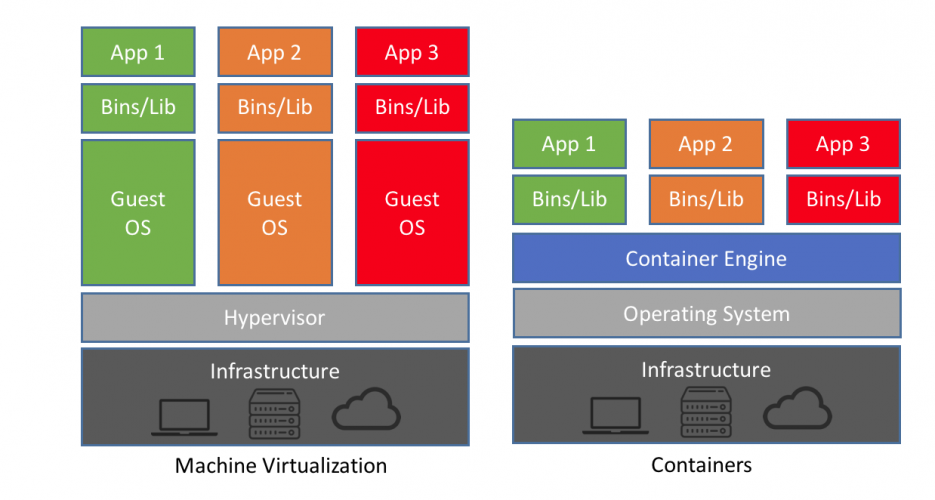
\includegraphics[width=0.8\textwidth]{bilder/comparison_vm_container.png}
        \label{fig:comparison_vm_container}
\end{figure}



\section{Open Container Initiative}
Die \ac{OCI} ist eine Organisation, die Standards für Container Runtimes und Formate erstellt.
Aktuell werden zwei Spezifikationen von der Organisation bereitgestellt, die \ac{runtime-spec} und die \ac{image-spec}.
Die Spezifikationen erlauben es verschiedener Software, das bereitgestellt Interface zu implementieren.
Die \ac{runtime-spec} definiert wie ein Container auf dem Host ausgeführt werden muss. 
Eine \ac{OCI}-Implementation, wie zum Beispiel Docker, lädt zum Ausführen eines Containers ein \ac{OCI}-kompatibles Container-Image herunter und entpackt dieses in ein Runtime Filesystem Bundle.
Ohne die Definitionen des \ac{OCI} könnte ein Container der im Docker-Format und die Docker-Runtime(\texttt{runc}) geschrieben wurde auch nur von Docker ausgeführt werden.
Die \ac{OCI}-Spezifikation ermöglicht es, mit jeder Container-Runtime, die \ac{OCI}-kompatibel ist, ein Docker-Image auszuführen. \cite{oci}



\section{Kubernetes}
Kubernetes ist eine \ac{FOSS}-Lösung zum managen von containerisierten Anwendungen.
Das System ermöglicht automatisches Skalieren und Deployen der Anwendungen, sowie integriertes Self-Healing, einfaches Management und Updaten.
Außerdem ist es vergleichsweise unproblematisch ein Kubernetes-Cluster selbst zu skalieren. 
Nodes lassen sich im Live-Betrieb nicht nur hinzufügen, sondern können genauso auch ausfallen. 
Die auf ihnen laufenden Container werden dann, wenn möglich ohne Downtimes, auf die verbliebenen zur Verfügung stehenden Nodes verteilt. 
Gehostet werden kann Kubernetes sowohl on-premise als auch in der public- oder hybrid-cloud.
\\
Entwickelt wurde die Technologie ursprünglich von Google, die schon seit 15 Jahren Produktions-Arbeitslast in Containern laufen lassen.
\cite{kubernetes}

\subsection{Cluster Komponenten}
\subsubsection{Proxy}
Der Proxy ist dafür verantwortlich, den Netzwerk-Verkehr zu Services in dem Kubernetes-Cluster zu routen. 
Dafür muss auf jeder Maschine des Clustern der entsprechende Proxy vorhanden sein, was mit der Kubernetes-Ressource \textit{DaemonSet} realisiert werden kann.
Diese sorgt dafür, dass auf jedem Node des Clusters der entsprechende Container läuft.\cite[S.34]{Kubernetes_up_and_running}
\subsubsection{DNS}
Der \ac{DNS}-Server ist für die Namensaulösung und die Entdeckung von Services innerhalb des Clusters verantwortlich. 
Der \ac{DNS}-Server selbst läuft als ein eigener Service in dem Cluster.
Damit er funktionieren kann, muss da Cluster mit einem funktionieren Container-Network ausgestattet sein. 
\cite[S.34 f]{Kubernetes_up_and_running}

\subsection{Container Runtime Interface}
In Kubernetes 1.5 wurde in Kubernetes das \ac{CRI} eingeführt.
Dieses Interface erlaubt es dem \texttt{kubelet} mit jeder Container Runtime zu arbeiten, die selbst dieses Interface implementiert. 
\texttt{Kubelet} kommuniziert über einen \texttt{shim} mit der Runtime, wobei der \texttt{shim} als Server funktioniert und \texttt{kubelet} als Client.
Der \texttt{\ac{CRI} shim} gibt dann die Befehle an die Runtime weiter, wie in Abbildung \ref{fig:cri} dargestellt.
\begin{figure}[ht]
        \caption{Kubernetes \ac{CRI}\cite{kubernetes_cri}}
        \centering
        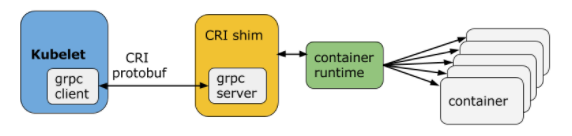
\includegraphics[width=\textwidth]{bilder/kubernetes_cri.png}
        \label{fig:cri}
\end{figure}
\cite{kubernetes_cri}

\subsection{Pods}
Ein Pod ist der kleinste Workload in einem Kubernetes Cluster, in ihm können ein oder mehrere Container laufen.
Wenn ein Pod-Manifest an die Kubernetes-\ac{API} geschickt wird, entscheidet der \texttt{sheduler} auf welchem der Nodes der Pod gestartet werden soll.
Gestartet und am Leben erhalten wird der Pod dann vom \textit{kubelet daemon}.
\cite[S.63]{Kubernetes_up_and_running}

\subsection{Service}
Das Service Objekt in Kubernetes wird benötigt um einen Service inner- oder außerhalb des Clusters zu exposen.
Services werden benötigt um verlässlich auf einen Pod zugreifen zu können.
Da sich in Kubernetes die Namen der einzelnen Pods bei jedem Neustart ändern können, wird ein gleichbleibendes Objekt benötigt, über das immer dieselbe dahinterliegende Applikation erreicht werden kann.
Diese Rolle übernimmt der Service.
Über Labels werden sie mit einzelnen Pods verknüpft und macht diesen so, über den Service, erreichbar.
\cite[S.86]{Kubernetes_up_and_running}

\subsection{Ingress}
Der Ingress leitet von \ac{HTTP} und \ac{HTTPS} Routes auf Services innerhalb des Clusters weiter.
Mithilfe dieser Ressource können Services mit \ac{URL}'s verknüpft werden, Load kann verteilt werden und \ac{SSL} / \ac{TLS} terminiert.
Beispielsweise können so \ac{URL}'s wie \textit{service1.host.com} und \textit{service2.host.com} zu den entsprechenden Services und Ports auf dem gleichen Host gemappt werden, wie in Abbildung \ref{fig:ingress} dargestellt.
\cite{kubernetes_ingress}
\begin{figure}[ht]
        \caption{Kubernetes Ingress\cite{kubernetes_ingress}}
        \centering
        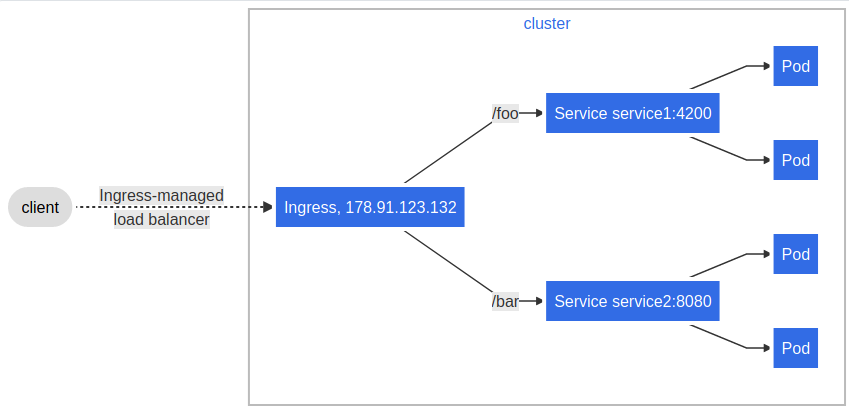
\includegraphics[width=\textwidth]{bilder/kubernetes_ingress.png}
        \label{fig:ingress}
\end{figure}

\subsection{Replica Set}
Ein Replica Set lässt sich als Pod-Manager beschreiben. 
In dieser Ressource kann definiert werden, wie viele Kopien von welchem speziellen Pod vorhanden sein sollen.
Das Replica Set wird dann immer dafür sorgen, dass genau so viele Kopien des Pods auf dem Cluster laufen wie deklariert. 
Wenn ein oder mehrere Pods sterben, die von einem Replica Set gemanagt werden, werden diese automatisch erneut gestartet. 
So lange bis wieder die gewünschte Anzahl an Pods erreicht ist.
Selbst wenn ein kompletter Node ausfällt, kümmert das Replica Set sich darum, dass der Pod auf einem anderen Node gestartet wird.
\cite[S.103 ff.]{Kubernetes_up_and_running}

\subsection{Deployment}
Das Deployment ist vor allem zum managen von neuen Software Releases gedacht. 
Durch den Rollout-Prozess wird es vereinfacht von einer Version der Software zur nächsten zu wechseln, zum Beispiel durch eingebaute Health-Checks die das Update anhalten wenn zu viele Instanzen der neuen Software-Version in einem Failed-State landen.
Durch Deployments können Downtimes komplett vermieden werden, indem von einer zu updatenden Software nach und nach die einzelnen Container durch Container mit der neuen Software Version ersetzt werden.
Wenn der letzte Container mit der alten Software-Version ersetzt wurde, ist das Update der Anwendungen ohne eine einzige Sekunde Downtime durchgeführt wurden.
Ein Deployment managt dazu Replica Sets, so wie diese die einzelnen Pods managen.
\cite[S.113 ff.]{Kubernetes_up_and_running}

\subsection{Stateful Set}
Stateful Sets sind ähnlich zu Replica Sets, haben aber einzigartige und eindeutige Eigenschaften.
Jede Kopie bekommt dazu einen persistenten Hostname, bei dem von 0 aufwärst hochgezählt wird. 
Wird das Stateful Set gelöscht, werden die Pods vom höchsten zum niedrigsten hin wieder gelöscht.
Durch den persistenten Namen ist es für andere Applikationen innerhalb des Clusters möglich immer genau die gleiche Instanz anzusprechen.
\cite[S.186 f.]{Kubernetes_up_and_running}

\subsection{Config Maps}
Eine ConfigMap wird genutzt um Konfigurations-Werte für eine Anwendungen zu setzen. 
Die gesetzen Variablen können das Environment das Containers definieren, mit dem sie verknüpft werden.
\cite[S.153]{Kubernetes_up_and_running}

\subsection{Secret}
Secrets sind sehr ähnlich zu Config Maps, mit dem einzigen Unterschied, dass die in ihnen gespeicherten Daten sensibel und deswegen verschlüsselt sind.
Das bedeutet, dass Sie sich für Passwörter, Security Token und secret Keys besser eigenen als Config Maps.
\cite[S.157 f.]{Kubernetes_up_and_running}

\subsection{Persistenter Storage}
Persistenter Storage in Kubernetes ist standartmäßig nicht gegeben. 
Die Plattform rechnet damit, dass die einzelnen auf ihr gehosteten Pods regelmäßig ausgetauscht zerstört werden. 
Um in so einem Umfeld persistenten Storage garantieren zu können gibt es in Kubernetes \ac{PV}s und \ac{PVC}s.

\subsubsection{Persistent Volume}
Ein \ac{PV} ist ein definierter Storage-Teil das mit einer Storage Class provisioniert wurde.
Ihr Lifecycle ist unabhängig von dem individuellen Pod der das \ac{PV} benutzt.

\subsubsection{Persistent Volume Claim}
Ein \ac{PVC} ist eine Anfrage des Users nach Storage.
In Ihnen werden Größe und Zugriffsart des benötigten Speicherplatzes definiert. 


\section{Kata-Runtime}
Das Kata Containers Projekt ist ein Open Source Projekt, das probiert die Vorteile beider zuvor erläuterten Technologien zu kombinieren.
Die Isolation von \ac{VM}s mit der Geschwindigkeit, dem geringen Management Aufwand und dem Self-Healing von Containern.
\\
Wenn ein Container-Image in der Kata-Runtime gestartet wird, wird tatsächlich kein Container gestartet, sondern eine lightweight \ac{VM} erstellt.
Diese hat ihren eigenen Kernel, der eine Isolation des Netzwerks, des Speichers und von \ac{I/O} garantiert, jedoch mit einem deutlich kleineren Overhead als konventionelle \ac{VM}s.
Um einen möglichst großen Anwenderbereich abzudecken arbeitet Kata nach den industriellen Standards \ac{OCI} und implementiert Kubernetes \ac{CRI}, das im Verlauf der Arbeit noch genauer geklärt wird. 
Durch die standardisierten Interfaces ist der Umstieg und das Arbeiten mit Kata in der Theorie sehr unkompliziert. \cite{kata}

\subsection{Geschichte}
Das Kata-Container Projekt entstand aus der Fusion von zwei vorhergehenden Projekten:
\begin{itemize}
        \item Clear Containers
        \\Dieses Projekt von Intel\footnote{https://www.intel.com/content/www/us/en/homepage.html} wurde 2015 ins Leben gerufen, um Sicherheitsbedenken beim Einsatz von Containern aus dem Weg zu räumen.
        Intel erschuf eine alternative Container Runtime, in der Container als minimale \ac{VM}s gestartet wurden, den Fokus setzten sie dabei auf Performance(<100ms boot time) und Sicherheit.\cite[S.1]{Kata_Containers}
        \item runV
        \\Ist ein ähnliches Projekt von der Firma "Hyper", die selbst eine Runtime entwickelt haben, die einen Hypervisor nutzt.
        Sie haben Ihren Fokus auf den Support vieler \ac{CPU}-Architekturen und Hypervisor gelegt.\cite[S.1]{Kata_Containers}
\end{itemize}
2016 hielten beide Firmen eine Präsentation über ihr jeweiliges Produkt auf der \say{Open Source Summit} in Berlin und wurden so aufeinander aufmerksam.
Ein Jahr später, in 2017, wurde beide Produkte unter der \ac{OSF} zu Kata-Containers zusammengeführt.\cite{kata_history}

\subsection{Vergleich mit traditionellen Containern}

\begin{figure}[ht]
        \caption{Vergleich von Kata-Containern und traditionellen Containern\cite{kata_learn}}
        \centering
        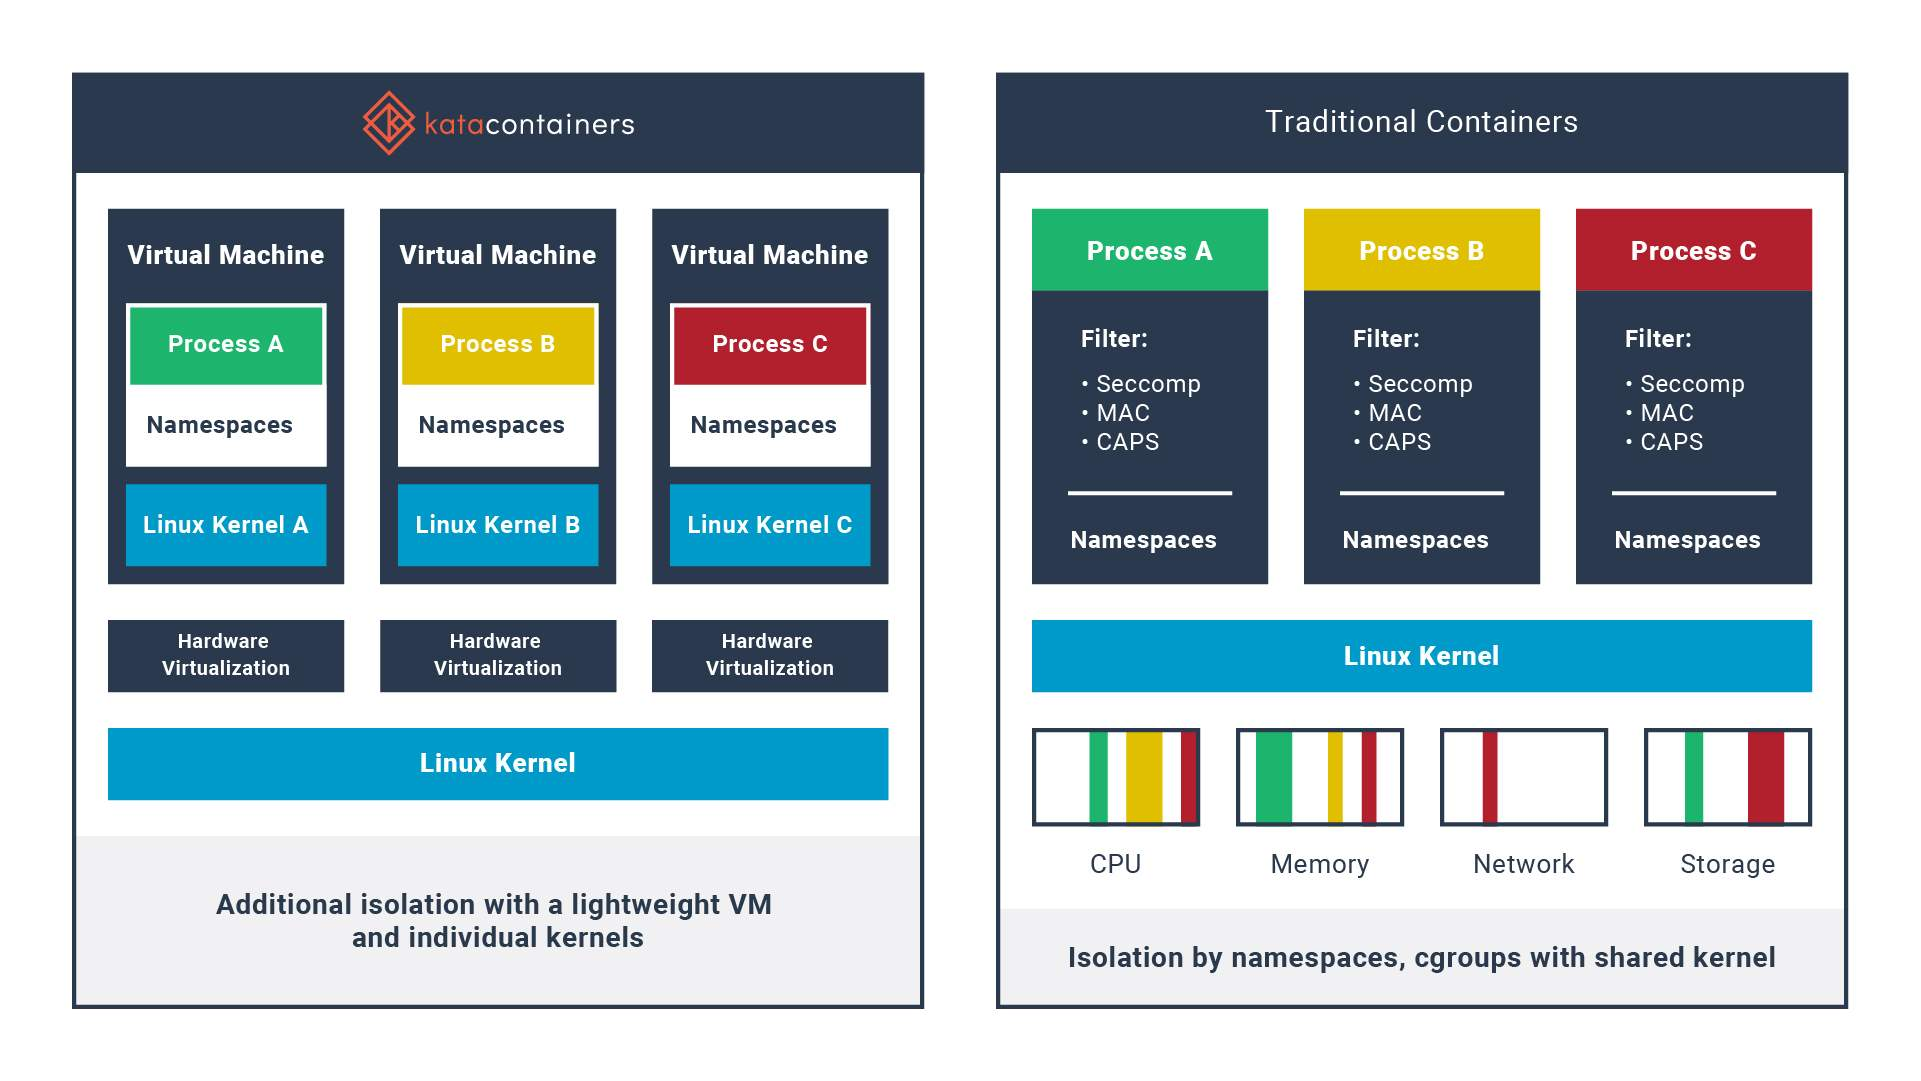
\includegraphics[width=\textwidth]{bilder/katacontainers_traditionalvskata_diagram.jpg}
        \label{fig:kata_vs_traditional}
\end{figure}

In der Abbildung \ref{fig:kata_vs_traditional} werden die wichtigsten Unterschiede dargestellt.
Traditionelle Container laufen alle auf demselben Kernel. 
Das bedeutet, dass jeder Container direkt auf den Ressourcen(\ac{CPU}, Memory, Network, Storage) des Hosts läuft. 
Eine Isolation wird durch Namespaces und cgroups realisiert.
\\
Bei den Kata-Containern hingegegen werden die Container in \ac{VM}s verpackt, von denen jede seinen eigenen Kernel bekommt.
Durch die Hardware-Virtualisierung kann jeder Container nur auf die Ressourcen zugreifen, welche für ihn erstellt wurden. 
In seinem Kernel laufen keine Prozesse, außer diejenigen der Applikation selbst.  

\subsection{Kata Container in Kubernetes}

\begin{figure}[ht]
        \centering
        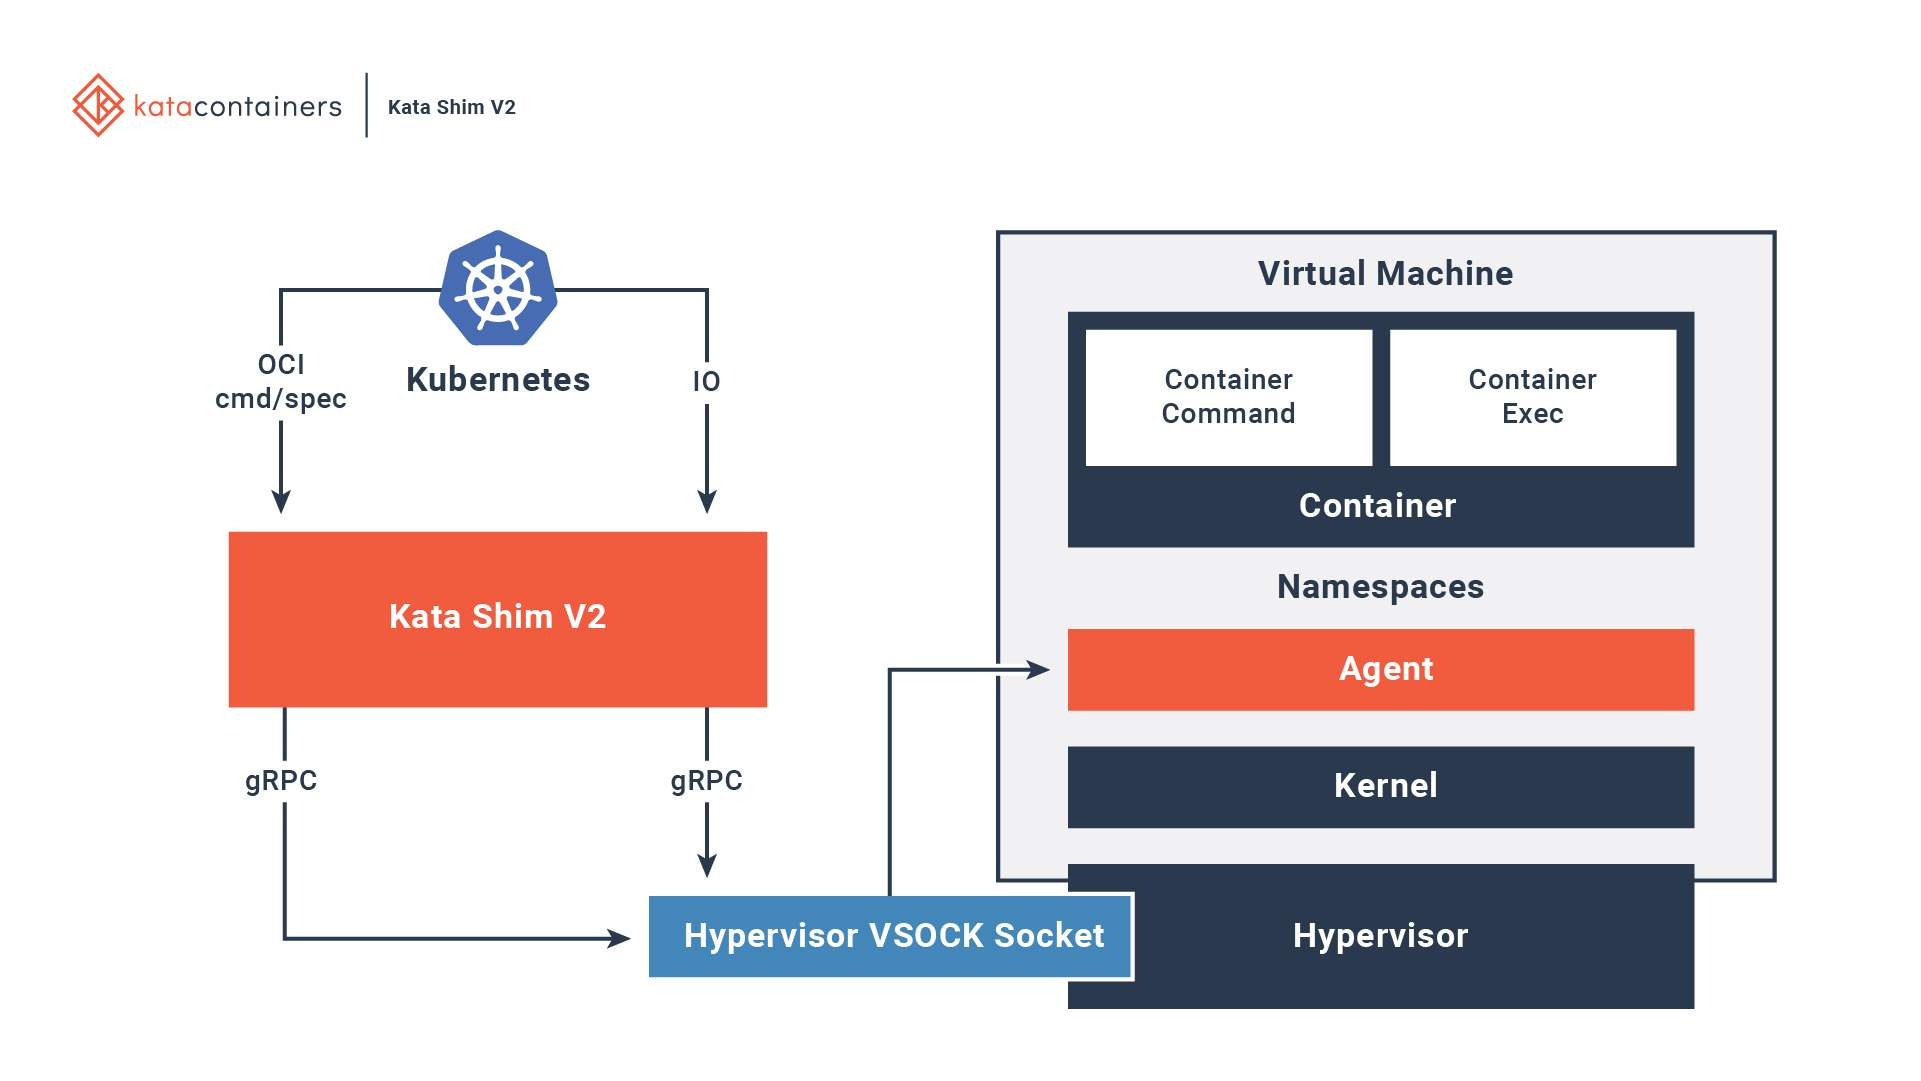
\includegraphics[width=\textwidth]{bilder/katacontainers_architecture_diagram.jpg}
        \caption{Kata Architektur\cite{kata_learn}}
        \label{fig:kata_architecture}
\end{figure}

In Abbildung \ref{fig:kata_architecture} lässt sich erkennen, dass eine Komponente namens \say{Kata Shim V2} eine große Rolle in der Kubernetes Integration spielt.
Kubernetes kann Pods und \ac{OCI}-kompatible Container mit dem \textit{kata-shimv2} starten. 
In der \ac{VM}, die von dem \textit{kata-shimv2} gestartet wurde, läuft unter anderem der \textit{kata-agent}, der für das Starten von Container-Prozessen eingesetzt wird.
Außerdem hostet er einen \ac{gRPC}-Server, über den der \textit{kata-shimv2} mit dem Agent in der \ac{VM} kommunizieren kann.
So können von dem Shimv2 Befehle zum managen von Containern in die Maschine gesendet werden, sowie \ac{I/O}-Streams transportiert werden, um so beispielsweise Commands in den Container auf dem Gast zu senden.
Auf diesem Weg werden aber genauso auch der \textit{stdout}- und \textit{stderr}-Stream an den \ac{CRI} Shim transportiert.
\cite{kata_architecture}

\todo{Kata mit Containerd in Kubernetes https://github.com/kata-containers/documentation/blob/master/how-to/containerd-kata.md}



\section{Ansible}
Ansible ist eine Software, mit dessen Hilfe Systeme deployed und gemanagt werden können. 
Dazu wird ein Prozess, der eigentlich händisch ausgeführt werden würde, in einem sogenannten Playbook abgebildet.
Dieses Playbook beschreibt der Reihe nach genau jede Bedingung die erfüllt sein muss, um den Prozess abzuschließen.
Durch die deklarative Natur von Ansible sind die Ergebnisse reproduzierbar und führen nur die Änderungen aus, die nötig sind.
Wird ein wiederkehrendes Problem einmal in einem Ansible-Playbook gelöst, kann dieses Playbook immer wieder Verwendung finden, wenn das Problem erneut auf einem ähnlichen System auftritt.
Ansible lässt sich auch einsetzen, um den Umgang mit bereits eingesetzten Technologien zu vereinfachen oder zu automatisieren.
\cite{ansible}

\subsection{Funktionsweise}
Ansible ermöglicht es, die gesamte Infrastruktur mitsamt all ihren Verbindungen zu beschreiben. 
So kann die ganze Umgebung, statt nur einzelne Systeme, auf einmal angepasst werden.
Dazu nutzt Ansible die bereits angesprochenen Playbooks, die in \ac{YAML} geschrieben sind, einer deklarativen und sehr simpel gestalteten Sprache.
\\
Wird ein Playbook ausgeführt stellt Ansible auf den einzelnen Systemen mithilfe von einigen Modulen den gewünschten Stand her, und löscht diese Module anschließend wieder. 
Um die Verbindungen zu den einzelnen Systemen herstellen zu können nutzt die Software standartmäßig \ac{SSH}-Keys, es sind allerdings auch andere Identity-Management Systeme wie z.B. Kerberos unterstützt.
Die Systeme selbst werden in den Inventory Files aufgelistet und können mit Gruppen und Variablen ausgestattet werden, um in einer Infrastruktur beispielsweise nur die Webserver oder nur die Datenbank-Server anzusprechen.
Wird ein OpenStack oder Ähnliches als Infrastruktur genutzt, kann sogar ein dynamisches Inventory generiert werden.
\cite{how_ansible_works}
\\
In diesem Projekt soll Ansible verwendet werden, um einen reproduzierbaren Weg zum installieren und konfigurieren der Kata-Runtime zu finden, sowie um das Kubernetes Cluster aufzubauen und zu managen. 


\section{Helm}
Helm ist eine Software, die das Installieren und Updaten von komplexen Kubernetes Applikationen vereinfachen soll.
Helm-Charts sind einfach zu erstellen, sie bieten eine gute Versionierung, lassen sich veröffentlichen und teilen, sowie templaten.
Das Projekt ist ein \ac{CNCF}-Projekt und wird von der Community gepflegt.
Charts beschreiben komplexe Applikationen und ermöglichen somit eine vereinfachte Installation von umfangreicher Software, außerdem sind diese einfach zu teilen und somit ein guter Weg um Software zu veröffentlichen.
\cite{helm}
\\
Für das \ac{SORMAS}-Projekt wird Helm jedoch auch vor allem wegen der guten Templating Möglichkeiten eingesetzt.
Verschiedene \ac{GAs} benötigen unterschiedliche Attribute, die alle über das Helm-Templating gesetzt werden könne.
So kann garantiert werden, dass nur an einer einzigen Stelle im Code jemals Anpassungen gemacht werden müssen, wenn eine neue \ac{SORMAS-ÖGD}-Instanz ausgerollt werden soll.
	\chapter{Praktischer Teil}
	\chapter{Ergebnisse}
	\chapter{Diskussion}
	\input{Kapitel/Fazit/Fazit}


	\bibliographystyle{alphadin} 
	\bibliography{literatur}
	
	\clearpage
	\appendix
	\pagenumbering{Roman}

\end{document}